\chapter{Survey and Taxonomy of Code-Based Crypto Art}
\label{chap:survey}

This chapter presents a survey of representative code-based crypto artworks, and provides a taxonomy that is relevant to the preservation of this type of art. Whilst not an exhaustive survey, this exercise was important for this study, because it provides relevant and applicable knowledge that informs the development of the artifact, and thus contributes to the research rigor, as specified by the DSR methodology discussed in \autoref{sec:methodology}.


\section{Survey of Code-Based Crypto Art}
\label{sec:survey-crypto-art}

\begin{figure}[h]
    \centering
    \captionsetup{justification=centering}
    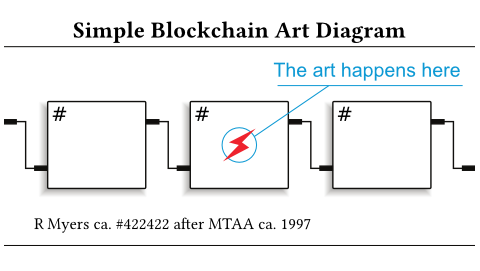
\includegraphics[width=0.50\linewidth]{simple-blockchain-art-diagram.png}
    \captionsetup{justification=centering}
    \caption[Simple Blockchain Art Diagram, by Rhea Myers]{Simple Blockchain Art Diagram, by Rhea Myers. \\ Source: https://rhea.art/simple-blockchain-art-diagram/}
    \label{fig:vdp}
\end{figure}



In the following section several code-based crypto artworks will be reviewed. They were selected for their unique properties, with the goal of providing a representative sample of the types of artworks available and helping understand the challenges that they pose from a preservation point of view.

\subsection{Configurable API Endpoints}

Stevie Jones, a.k.a. 1x1\footnotemark[1], a multi-instrumentalist, producer and coder originally from Northern Ireland, produced some of the earliest music NFTs. He also pioneered the use of an interactive options menu on OBJKTs which allows the user to modify the IPFS endpoint domain name on the artwork's UI, hence dealing with the mutable dependency dilemma directly on the OBJKT. This was the case with one of his early albums minted as an OBJKT on HEN, Fragments from The Cross, Vol. 3, see \autoref{fig:1x1_cross}.

Interestingly this piece also makes a request to \texttt{api.better-call.dev}, an endpoint which is no longer available. Stevie explained, in a personal communication, that the request was to check if the viewer owned two previous editions of the series, in which case additional content would be unlocked. From a preservation perspective, the challenge with this piece is the fact that it is fully interactive, and it requires clicking on each track to initiate the respective network request. A single automated snapshot archive of this OBJKT will be highly incomplete, as it will be missing all the media.

\footnotetext[1]{\url{https://1x1-music.com/}}

\begin{figure}[H]
  \centering
  \captionsetup{justification=centering}
  \begin{subfigure}[b]{0.45\textwidth}
    \centering
    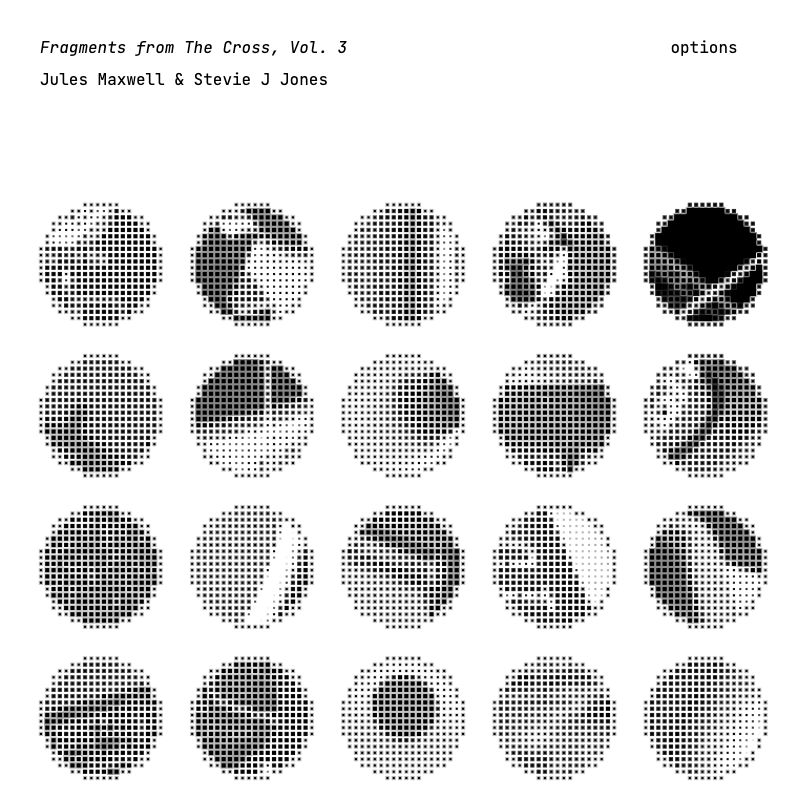
\includegraphics[width=\textwidth]{fragments-cross-main.png}
    \caption{Front Cover}
    \label{fig:vdp1}
  \end{subfigure}
  \hfill
  \begin{subfigure}[b]{0.45\textwidth}
    \centering
    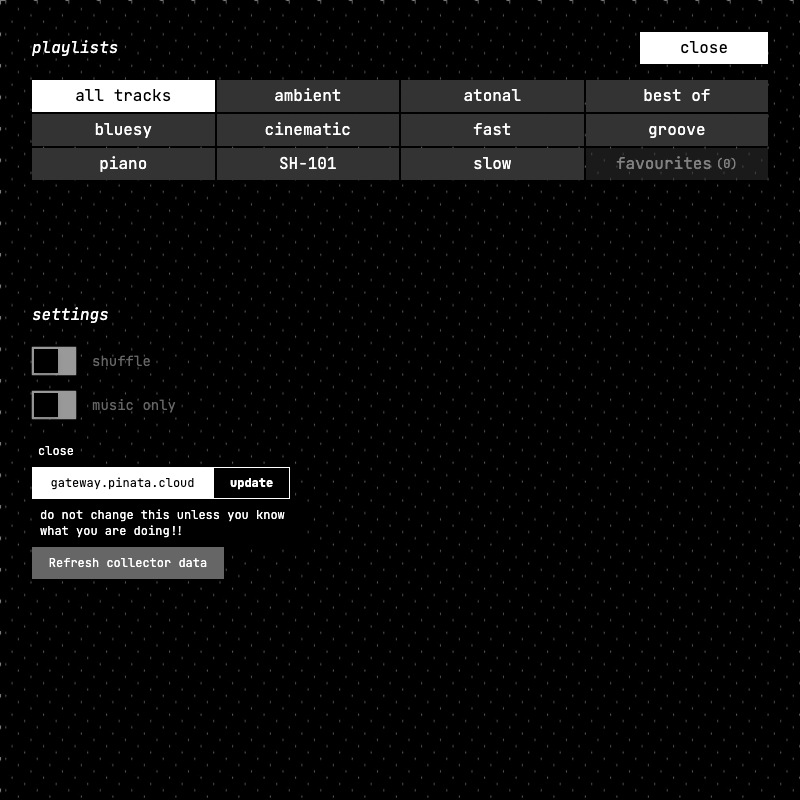
\includegraphics[width=\textwidth]{fragments-cross-menu.png}
    \caption{Options UI, with IPFS URL config}
    \label{fig:vdp2}
  \end{subfigure}
  \caption[Fragments from The Cross, Vol. 3]{Fragments from The Cross, Vol. 3 by Jules Maxwell \& Stevie Jones. \\ Source: https://teia.art/objkt/83079}
  \label{fig:1x1_cross}
\end{figure}


\subsection{Requests to Private Servers}

\begin{figure}[h]
    \centering
    \captionsetup{justification=centering}
    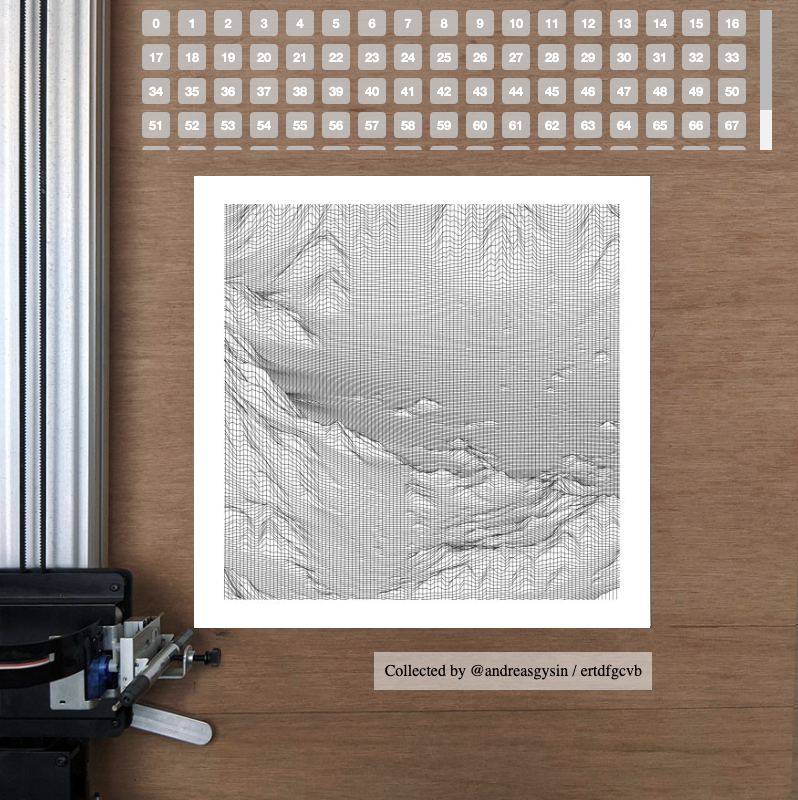
\includegraphics[width=0.75\linewidth]{possible-landscape.png}
    \captionsetup{justification=centering}
    \caption[a possible landscape by Joanie Lemercier]{a possible landscape by Joanie Lemercier. \\ Source: https://teia.art/objkt/33076}
    \label{fig:vdp}
\end{figure}

In a groundbreaking conceptual piece within the context of HEN, Joanie Lemercier\footnotemark[2], linked the act of collecting the piece with the drawing of a physical plotter landscape, which would be revealed within the OBJKT itself. Minted at a time when there were no restrictions on network request destinations, Lemercier uses requests to his own personal domain, \texttt{https://joanielemercier.com}, to load the assets for each print completed. Similarly to Stevie's Fragments of a Cross, it only initiates these requests when a user interacts with the piece.

Since, according to Lemercier, this piece is now ``completed'', one single full snapshot, including the recording/archival of each and every landscape would suffice. This is is an important intervention as the assets in the private server are at much higher risk than assets stored in IPFS.

\footnotetext[2]{\url{https://joanielemercier.com/}}

\begin{figure}[h]
    \centering
    \captionsetup{justification=centering}
    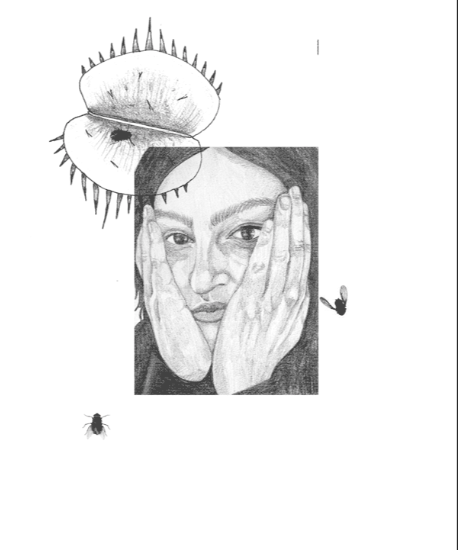
\includegraphics[width=0.50\linewidth]{becoming-body.png}
    \captionsetup{justification=centering}
    \caption[Becoming-body by Jessica Luz and Carlos de Oliveira Junior]{Becoming-body by Jessica Luz and Carlos de Oliveira Junior. \\ Source: https://teia.art/objkt/168794}
    \label{fig:becoming-body}
\end{figure}

\subsection{Requests to Indexers}

Several networked HEN OBJKTs made use of requests to indexers, to retrieve the list of collectors, amount spent on the artwork, and other blockchain or market related data.
We already mentioned ``Planned Obsolescence'' by Mario Klingemann, see page \pageref{fig:plannedobsolescence}.

``Becoming-body'', a collaboration between Brazilian artists Jessica Luz\footnotemark[3] and Carlos de Oliveira Junior (a.k.a. @vamoss\footnotemark[4]), was created within the TIBUM residency. The artwork contains a series of 36 animated GIFs, which will swap each time the artwork is collected, see \autoref{fig:becoming-body}.

\footnotetext[3]{\url{https://linktr.ee/jessicaluz___}}
\footnotetext[4]{\url{https://vamoss.com.br/}}


\subsection{Requests to RPC nodes}

Yazid\footnotemark[5], an artist and technologist from Brunei, has authored several networked NFTs, both as OBJKTs on HEN as well as in other blockchains. In his piece ``OBJKTs (Mondrian Edition)'', Yazid abandoned the dependency on indexers in favour of embedding the Taquito JS library, which enabled the piece to contact the RPC nodes directly. In addition to cycling through 2 RPC endpoints for extra resiliency, the RCP API is also more stable than indexer APIs. A testament to this resiliency is the fact that this OBJKT still works today. The OBJKT queries the blockchain every minute for the latest OBJKT ID minted, and represents it as a series of bars in a Mondrian style, each column representing a digit of the number. See \autoref{fig:mondrian}. This means the artwork evolves rather quickly, with the rendering changing each time another OBJKT gets minted, in real time.

\footnotetext[5]{\url{https://linktr.ee/__yazid__}}

\begin{figure}[h]
    \centering
    \captionsetup{justification=centering}
    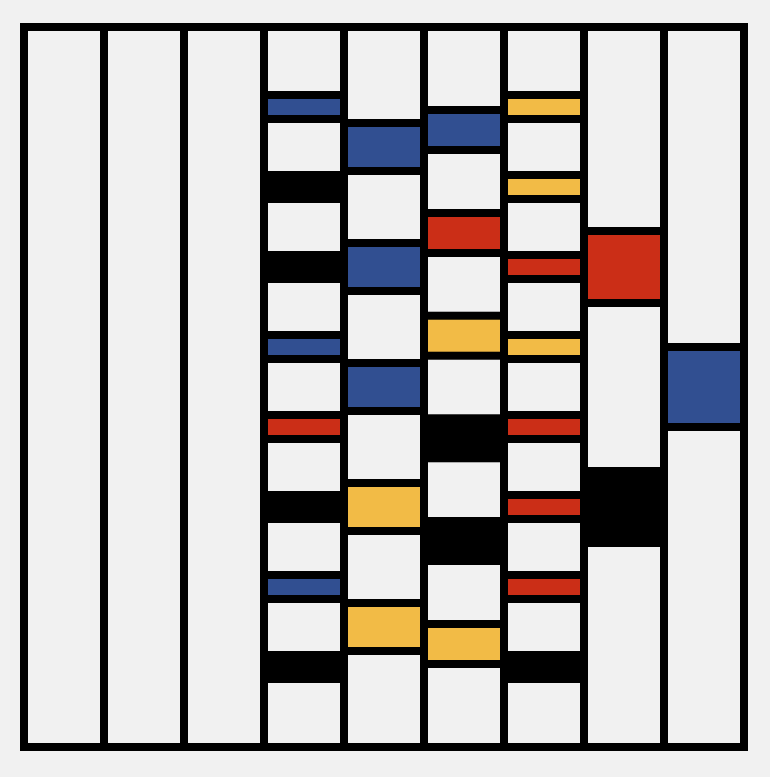
\includegraphics[width=0.50\linewidth]{objkts-mondrian.png}
    \captionsetup{justification=centering}
    \caption[OBJKTs (Mondrian Edition) by Yazid]{OBJKTs (Mondrian Edition) by Yazid. \\ Source: https://arkivo.art/artifacts/HEN/200599}
    \label{fig:mondrian}
\end{figure}

London-based James Bloom\footnotemark[6] (a.k.a. crashblossom) is another artist known for his blockchain-interactive artworks. Using a mixture of requests to configurable RPC endpoints and private infrastructure, James creates artworks that react in real-time to changes in the blockchain. Mass, a blockchain-interactive artwork minted on Ethereum, is particularly interesting because the artwork monitors every action its owners take on-chain, and uses that data to enact changes in the rendered 3D space, in what James calls a "mass surveillance machine", see \autoref{fig:mass}.

Preserving these types of blockchain-interactive artworks requires the preservation of the blockchain on which they depend, or at least snapshots of the blockchain data at given points in time, allowing for the replaying of the network calls initiated by the artwork's code.

\footnotetext[6]{\url{https://crashblossom.co/}}

\begin{figure}[h]
    \centering
    \captionsetup{justification=centering}
    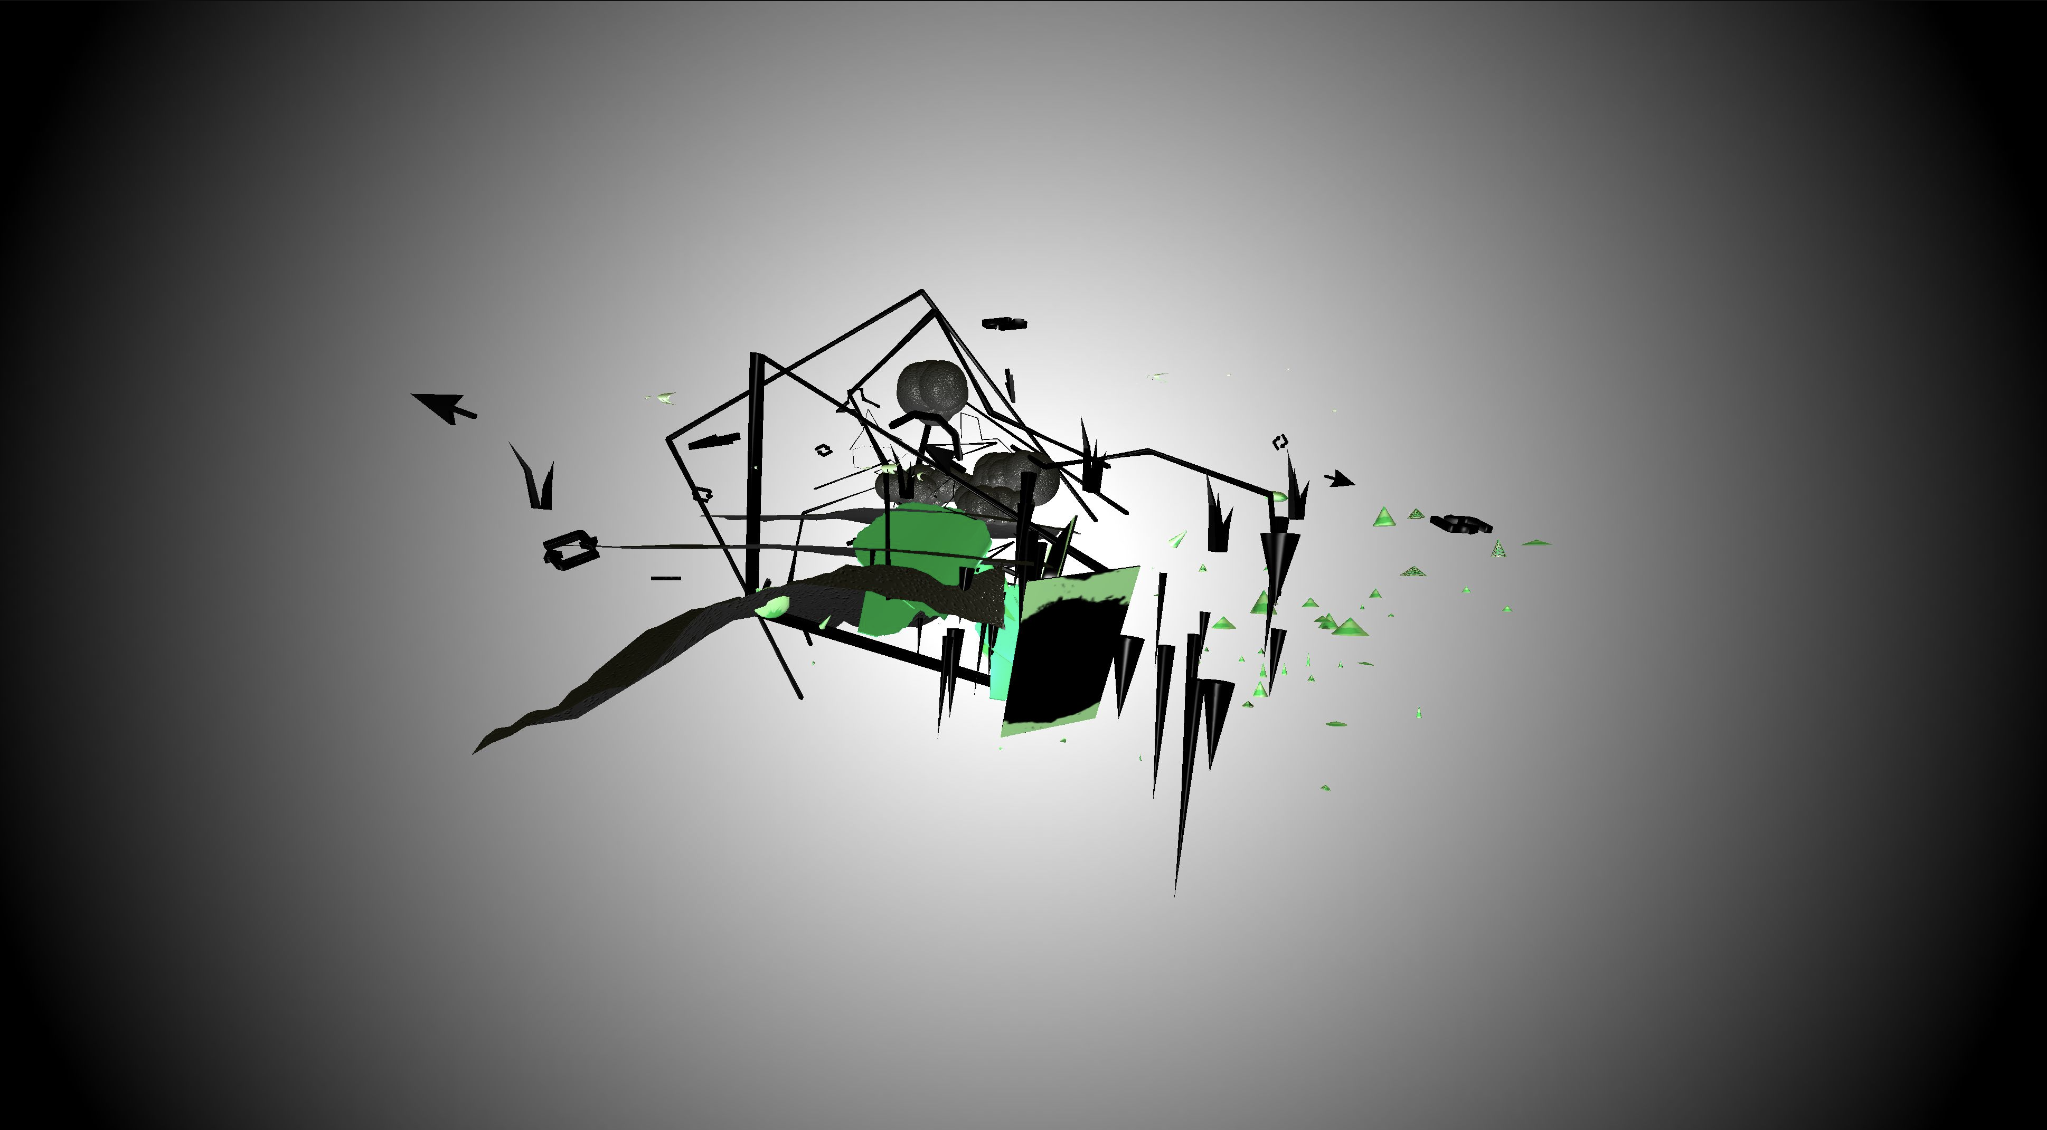
\includegraphics[width=0.75\linewidth]{mass.png}
    \captionsetup{justification=centering}
    \caption[Mass \#1 by James Bloom]{Mass \#1 by James Bloom. \\ Source: https://opensea.io/assets/ethereum/ \\
    0x80faa45d6f6cbdafdeba2f9c4a0237f74e5d8d9c/1}
    \label{fig:mass}
\end{figure}


\subsection{Custom Renderings Based on Ownership}

Another common theme amongst code-based OBJKTs is the customisation of the rendering based on whether the viewer owns the artwork. The piece can tell the Tezos wallet address of the viewer because, if the user is logged in to Teia, it passes their wallet address to piece via URL query parameters. The piece then can query the blockchain to determine if that address owns any editions of itself, or even of other OBJKTs.

Raphaël de Courville\footnotemark[7] (a.k.a. sableraph), a French generative artist and creative coder based in Berlin, has experimented with this idea in two conceptual artworks. The first one, Adam, consults the blockchain (via the hicdex indexer) and gathers how many editions of the artwork have been sold, data which it uses to start erasing itself gradually. However at the same time it also checks how many editions of the artwork the viewer owns, and modifies the rendering slightly for them. These changes are subtle, resulting in a slow evolution over time, see \autoref{fig:adam}.

\footnotetext[7]{\url{https://linktr.ee/sableraph}}

\begin{figure}[h]
    \centering
    \captionsetup{justification=centering}
    \fcolorbox{gray}{white}{
\includegraphics[width=0.75\linewidth]{adam-full.png}}
    \captionsetup{justification=centering}
    \caption[Adam by Raphaël de Courville]{Adam by Raphaël de Courville. \\ Source: https://teia.art/objkt/230177}
    \label{fig:adam}
\end{figure}


\begin{figure}[H]
  \centering
  \captionsetup{justification=centering}
  \begin{subfigure}[b]{0.45\textwidth}
    \centering
    \fcolorbox{gray}{white}{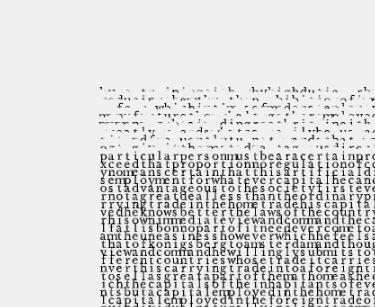
\includegraphics[width=\textwidth]{adam-no-own.png}}
    \caption{Viewer does not own OBJKT}
    \label{fig:adam-no-own}
  \end{subfigure}
  \hfill
  \begin{subfigure}[b]{0.45\textwidth}
    \centering
    \fcolorbox{gray}{white}{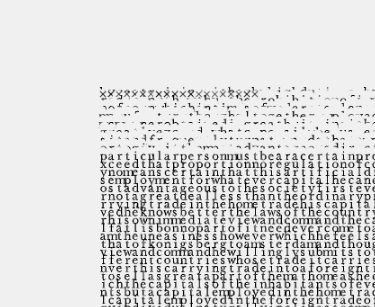
\includegraphics[width=\textwidth]{adam-own.png}}
    \caption{Viewer owns 5 editions of OBJKT}
    \label{fig:adam-own}
  \end{subfigure}
  \caption[Detail of Adam by Raphaël de Courville (sableraph)]{Detail of Adam by Raphaël de Courville (sableraph). \\ Source: https://teia.art/objkt/230177}
  \label{fig:adam-detail}
\end{figure}

The second, a collaboration with Malaysian artist Mumu\footnotemark[8], ``Moon's medication: Your meditation'', explores the relationships between 2 OBJKTs. Instead of changing itself based on the number of editions that the viewer has of this OBJKT, it checks how many editions the viewer collected of another OBJKT, ``Moon's medication - Day'', and starts adding coloured medication tabs, with the number of colours reflecting the number of editions the viewer owns: red, orange, yellow, green, blue and purple, see \autoref{fig:moon-med}.

\footnotetext[8]{\url{https://linktr.ee/mumu_thestan}}

\begin{figure}[H]
  \centering
  \captionsetup{justification=centering}
  \begin{subfigure}[b]{0.45\textwidth}
    \centering
    \fcolorbox{gray}{white}{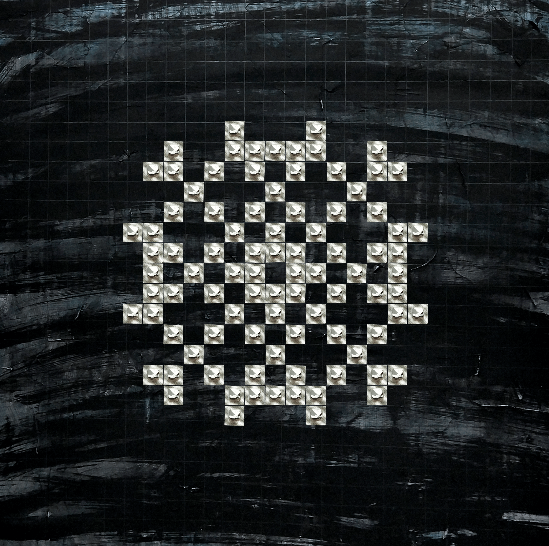
\includegraphics[width=\textwidth]{moons-med-no-own.png}}
    \caption{Viewer does not own Moon's medication - Day}
    \label{fig:adam-no-own}
  \end{subfigure}
  \hfill
  \begin{subfigure}[b]{0.45\textwidth}
    \centering
    \fcolorbox{gray}{white}{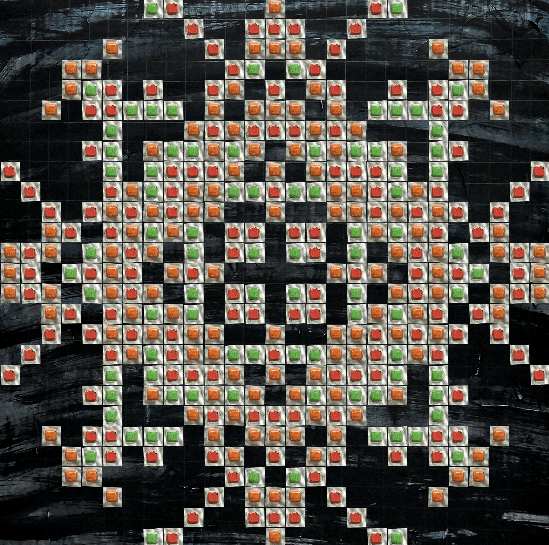
\includegraphics[width=\textwidth]{moons-med-own.png}}
    \caption{Viewer owns 3 editions of Moon's medication - Day}
    \label{fig:adam-own}
  \end{subfigure}
  \caption[Moon's medication : Your meditation]{Moon's medication: Your meditation by Raphaël de Courville (sableraph) and Mumu. \\ Source: https://teia.art/objkt/631387}
  \label{fig:moon-med}
\end{figure}


\subsection{Time/System Clock Based Art}

\begin{figure}[h]
    \centering
    \captionsetup{justification=centering}
    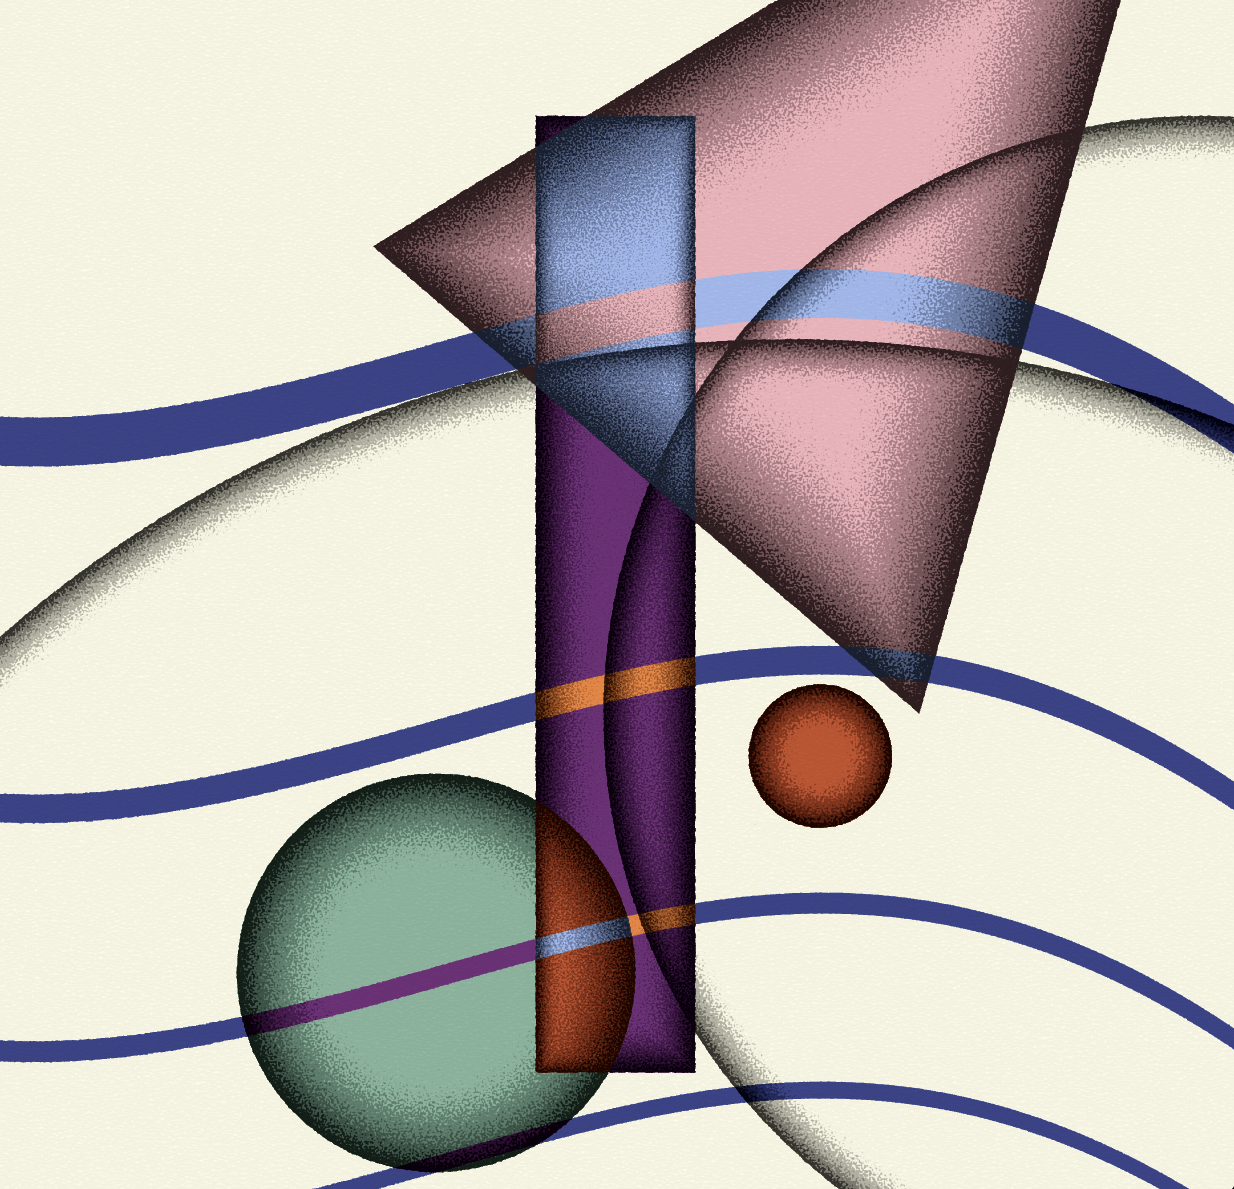
\includegraphics[width=0.50\linewidth]{detachment.png}
    \captionsetup{justification=centering}
    \caption[Detachment by Thomas Lin Pedersen]{Detachment by Thomas Lin Pedersen. \\ Source: https://thomaslinpedersen.art/work/detachment/}
    \label{fig:detachment}
\end{figure}

Code-based artworks that evolve deterministically, based purely on the system clock, have a very interesting preservation property: their complete evolution, which in theory can span thousands of years, is entirely encapsulated and self-contained in the code. Since all you need to provide the artwork with is the system time, you can in theory rewind or fast-forward hours, days, weeks, or centuries in an instant.

Thomas Lin Pedersen\footnotemark[9], a software engineer and generative artist from Denmark, encapsulated this philosophical concept of time-based determinism in his piece, Detachment, see \autoref{fig:detachment}. The artwork is in perpetual slow motion, and one that is deterministically tied to the current time.
Another interesting property of this kind of artwork is that any two viewers who open the artwork at the same time, as long as their device clocks are synchronised, will visualise the exact same rendering, even across different timezones, as the artwork uses the Coordinated Universal Time (UTC) time zone.

\footnotetext[9]{\url{https://thomaslinpedersen.art/}}

One can theorise that time-based artworks are, in fact, networked. However, instead of initiating a network request to an external API, they simply consult the API locally, which in JavaScript is as simple as: \texttt{new Date()}. The computer system in turn keeps that ``data source'' (the system clock) up-to-date by using external time servers (NTP), which keep the computers and other devices synchronised across the world.

Having said that, as tempting as it is to classify time-based artworks as networked, the fact is that they have very different conservation needs from the other kind of networked artwork that we examined before.


\subsection{Browser LocalStorage Interaction}

Several code-based artworks interact with the Browser's LocalStorage system, normally to persist configuration options. However Bjørn Staal\footnotemark[10] (a.k.a. nonfigurativ), an artist, programmer, and researcher from Norway, adopted this LocalStorage as an art medium, and produced Entangled. This remarkable artwork consists of a collection of 512 editions, minted on Ethereum (256 editions) and Tezos (256 editions) through the fxhash platform. Each of the editions is randomly paired with another across the two blockchains, and when one of these pairs are opened on the same browser instance (as small floating windows on the same web page) they interact with each other, using the LocalStorage as a way to coordinate their relative X,Y positions on the screen.

\footnotetext[10]{\url{https://linktr.ee/nonfigurativ}}

\begin{figure}[h]
    \centering
    \captionsetup{justification=centering}
    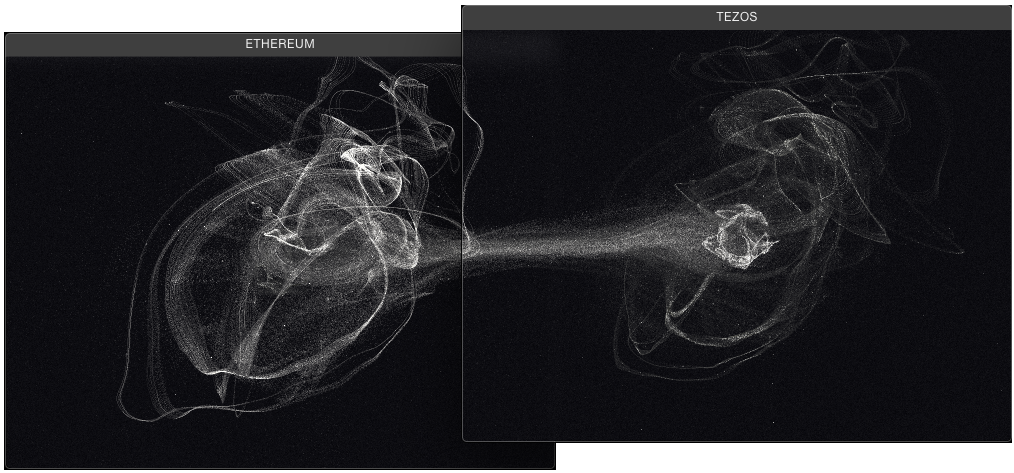
\includegraphics[width=0.75\linewidth]{entangled.png}
    \captionsetup{justification=centering}
    \caption[Entangled by Bjørn Staal]{Entangled by Bjørn Staal. \\ Source: https://www.fxhash.xyz/vertex/entangled}
    \label{fig:detachment}
\end{figure}


\subsection{Self-Contained Data}

All code-based artworks are in a way, data-driven. However all of the artwork types presented above require interacting with an external system for gaining access to that data, even if indirectly as is the case of the time-based artwork.

Javier Graciá Carpio\footnotemark[11] (a.k.a. jagracar), an astronomer, researcher, and creative coder from Spain, created several data-driven artworks that package their data with the artwork's assets, therefore reducing its dependency on external APIs. This does mean the artwork's evolution is limited to the data available to it at the time of minting. The benefit is that it makes for a very resilient artwork, with very simple preservation requirements. One such example is ``50461 users in hic et nunc'' which draws from a wide range of market activity to represent connections between users of HEN, see \autoref{fig:hen-users}. It should be noted that this artwork is user-interactive, which does increase the complexity of preservation.

\footnotetext[11]{\url{https://jagracar.com/}}


\begin{figure}[H]
    \centering
    \captionsetup{justification=centering}
    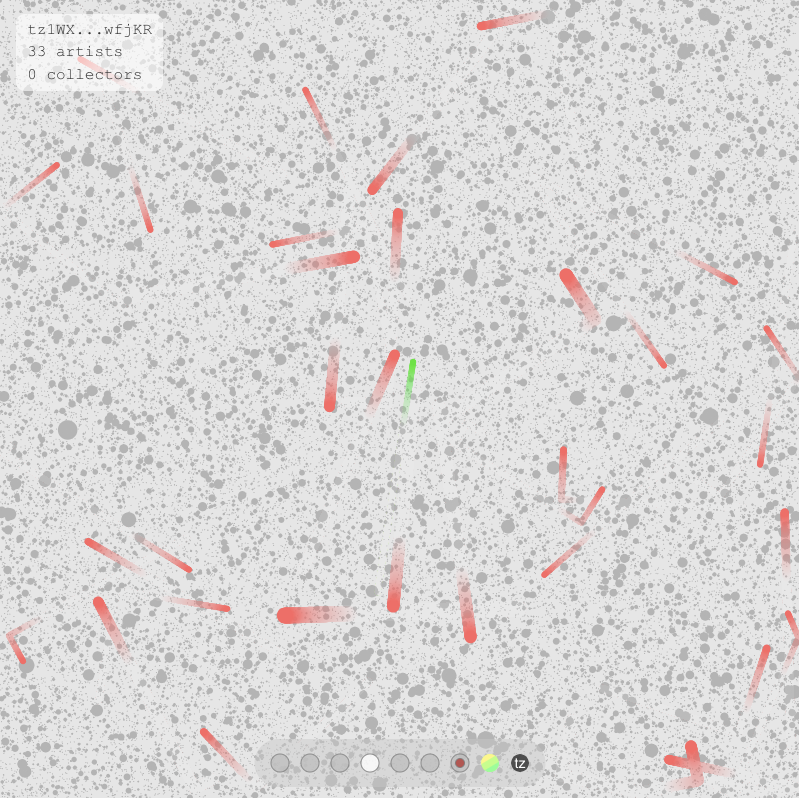
\includegraphics[width=0.50\linewidth]{hen-users.png}
    \captionsetup{justification=centering}
    \caption[50461 users in hic et nunc by Javier Graciá Carpio]{50461 users in hic et nunc by Javier Graciá Carpio. \\ Source: https://teia.art/objkt/427089}
    \label{fig:hen-users}
\end{figure}


\subsection{Determinism}

This section deals with whether artworks are deterministic in the way they are rendered or whether there is an element of randomness that even given all the same starting conditions, the artwork will look very different each time. This categorisation is important for conservation because a nondeterministic artwork will be difficult to monitor from a browser obsolescence point of view, especially when using image difference between consecutive snapshots of the artwork. In the case of a non-deterministic artwork, the snapshots will be so different that they become ineffective in detecting changes due to browser version upgrades or other changes in web specifications overtime. In this context, the challenge is to differentiate between a deterministic animated artwork, and a nondeterministic artwork. This challenge exists, because even if an artwork is deterministic, unless there is a way to snapshot the exact same frame across all the snapshots then any image difference comparisons will result in exaggerated differences. In this case we may need to employ more advanced animation frame comparison algorithms, such that the sequence of the animation can be compared across snapshots, and these may involve the recording of the animation, rather than just taking a single snapshot in time. Of course, such a strategy has trade-offs, and in this particular case the trade-off would be a much larger snapshot file size, which will then impact on the overall economic sustainability of the archive.

An example of non-deterministic artwork is Entropic, by generative art coding group united(fx)\footnotemark[12]. Each time the generative artwork is refreshed, a new random seed is used, resulting in a completely different output, see \autoref{fig:entropic}.

\footnotetext[12]{\url{https://unitedfx.xy}}

\begin{figure}[h]
    \centering
    \captionsetup{justification=centering}
    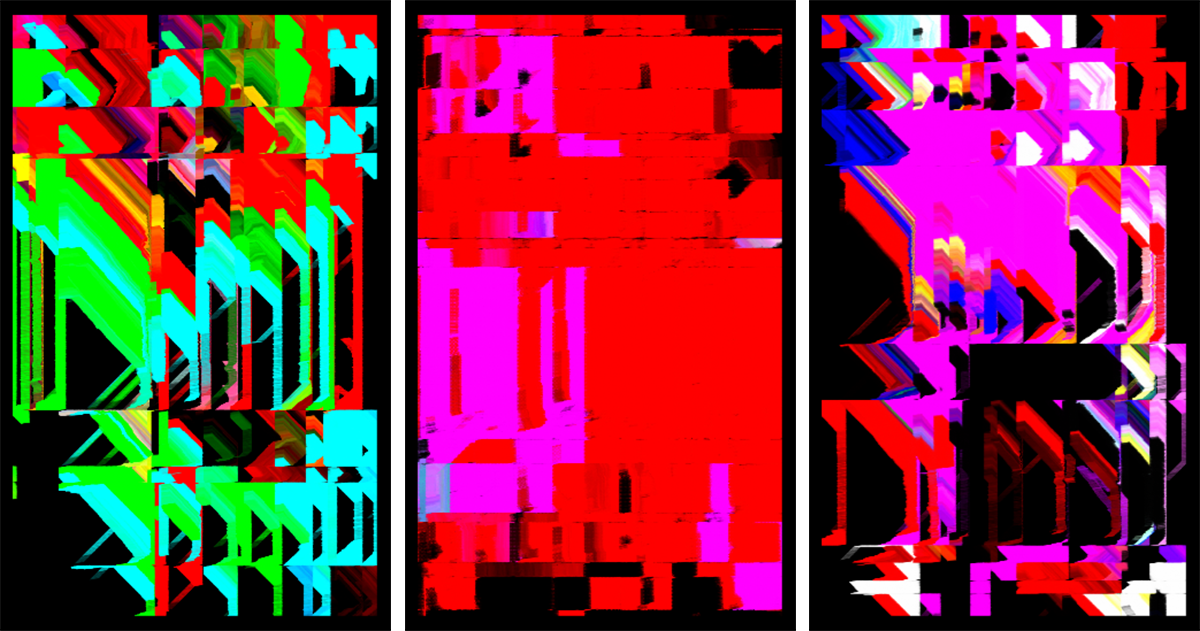
\includegraphics[width=0.75\linewidth]{entropic.png}
    \captionsetup{justification=centering}
    \caption[Entropic by united(fx) - 3 Renderings]{Entropic by united(fx) - 3 Renderings. \\ Source: https://teia.art/objkt/853589}
    \label{fig:entropic}
\end{figure}


It should be noted that, determinism is also a reason why fxhash moderates any networked NFT minted on their platform. For example, Australian artist Kath O'Donnell (a.k.a. aliak)\footnotemark[13] saw her networked data-driven artwork ``Data as Landscape'' moderated for this reason, see \autoref{fig:aliak-data-as-landscape}.


\footnotetext[13]{\url{http://aliak.com/}}


\begin{figure}[h]
    \centering
    \captionsetup{justification=centering}
    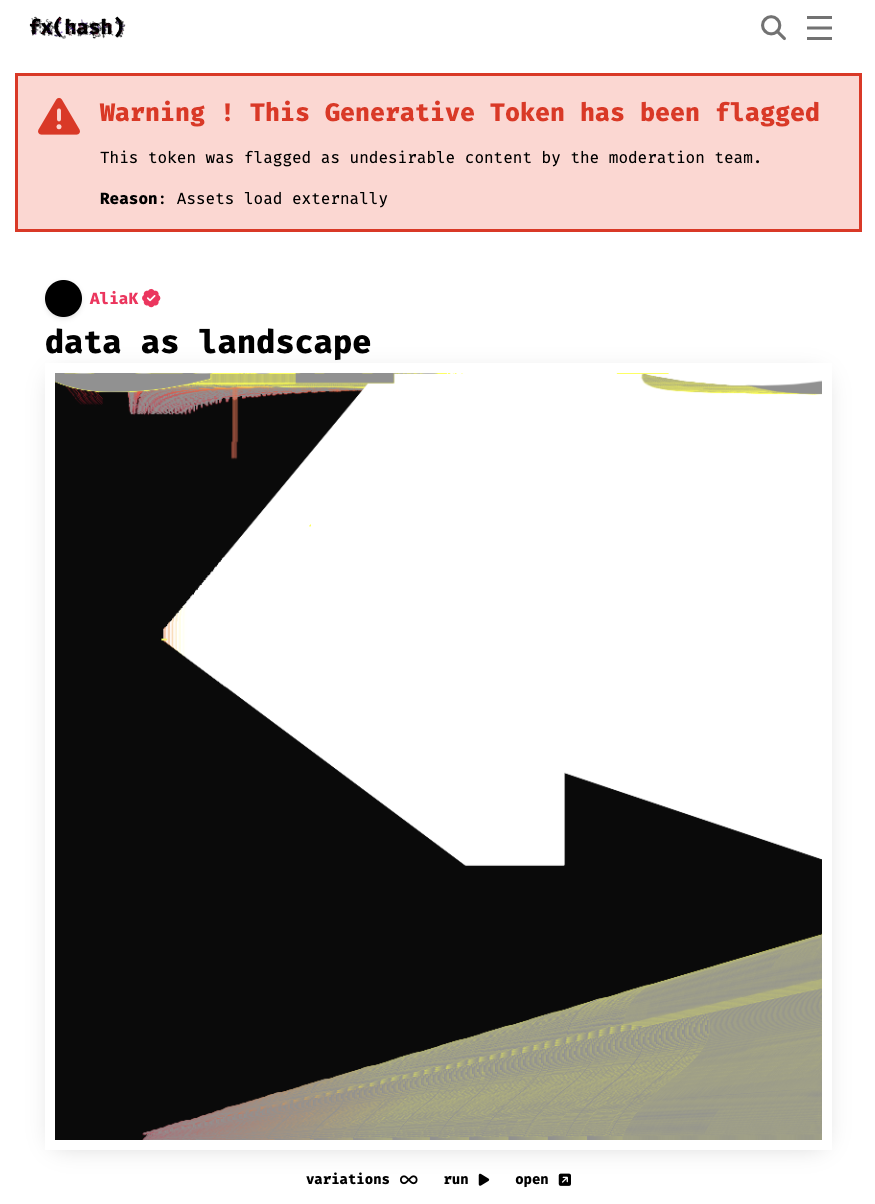
\includegraphics[width=0.5\linewidth]{aliak-data-as-landscape.png}
    \caption[Data as Landscape by AliaK]{Data as Landscape by AliaK, 2022. Source: https://www.fxhash.xyz/generative/13124}
    \label{fig:aliak-data-as-landscape}
\end{figure}



\section{Tentative Taxonomy of Code-Based Crypto Art}
\label{sec:interactivity}

When looking at the preservation of code-based crypto art, it is useful to be able to classify each artwork according to a taxonomy that informs conservators of the specific conservation methods that may be required at a later stage.

There is a clear lack of such a taxonomy in academic literature. Members of the crypto community have started efforts to classify code-based crypto art, such as Chainleft, see \autoref{fig:onchainruntimeart}.

\begin{figure}[h]
    \centering
    \captionsetup{justification=centering}
    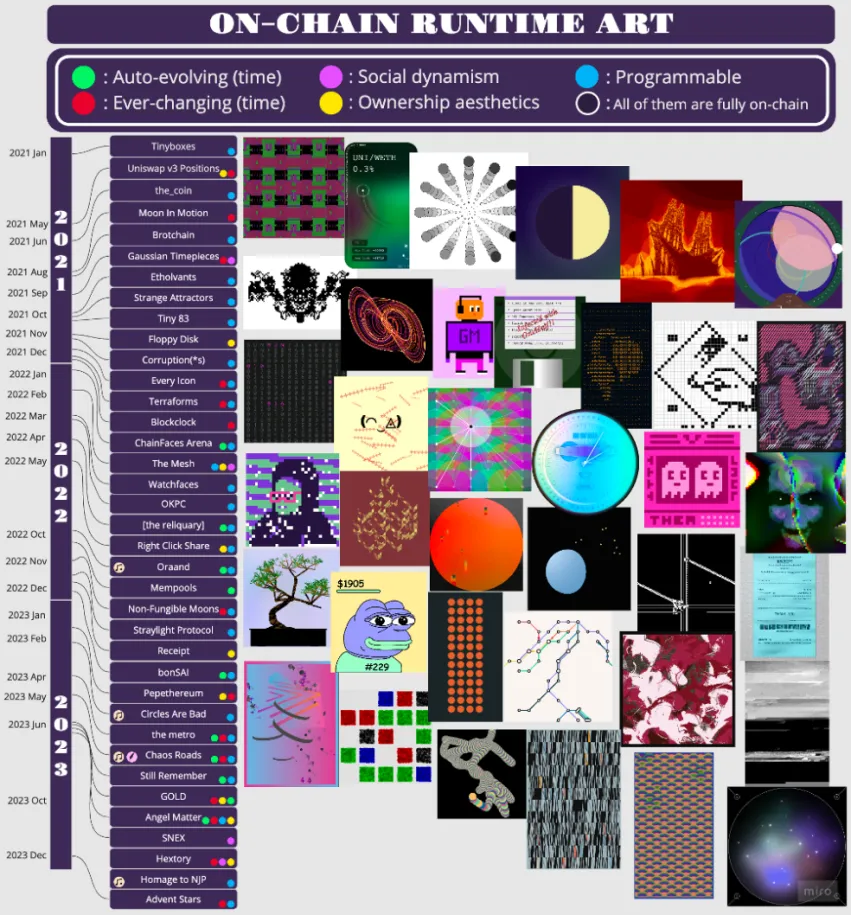
\includegraphics[width=0.75\linewidth]{chainleft-taxonomy.png}
    \caption[Onchain Runtime Art]{Onchain Runtime Art by @chainleft. Source: https://x.com/ChainLeftist/status/1757802497626767455}
    \label{fig:onchainruntimeart}
\end{figure}

Chainleft kindly shared a more detailed description of each category by private message, which can be found in \nameref{appx:chainleft-taxonomy}, page \pageref{appx:chainleft-taxonomy}. This is a good starting point for developing a taxonomy, however this study requires more fine-grained categorisation for certain technical elements of an artwork. 

For this study we will start by proposing that all code-based art is, fundamentally, data-driven. This may fall outside the traditional idea of data-driven art, which is more often linked with data visualisations. The fact is that no code may run without the use of data stored in variables, and these variables maintain the internal state of the artwork. The artwork's visual rendering is only possible by materialising this internal state into visual elements on the canvas. The question then is how that data originates and which interactions cause it to change in a way that justifies capturing it from a preservation perspective.


\begin{figure}[h]
    \centering
    \captionsetup{justification=centering}
    \includesvg[width=\textwidth]{code-based-art-interaction.svg}
    \caption[Code-Based Art Interaction Channels]{Code-Based Art Interaction Channels}
    \label{fig:code-based-art-interactions}
\end{figure}

\subsection{User Interaction}

The most common kind of interaction is user interaction, through the canvas and the usual input devices. This interaction may cause the artwork to change significantly from an aesthetic perspective, but it's a private experience between the user and the artwork. It is also more than likely an ephemeral interaction, without long-lasting effects on the artwork's state. As soon as the user closes the page or browser, the changes to the artwork's state are gone, and next time the user opens the artwork, it is back to its original state. The only exception to this is if the artwork saves state on the browser's LocalStorage or IndexedDB, causing it to persist between browsing sessions. Even then, this interaction is personal to the user, and does not affect the state of the artwork for other users.

The implication of this for preservation is that the recording of a user-interactive artwork should be orchestrated to also capture some of those interactions. This is a complex task to automate.

\subsection{Time Interaction}

As mentioned above, time or system clock interaction is the easiest to capture, because all the that conservator or capturing tool need are the original artwork's assets. Then it is just a matter of manipulating the time supplied to the artwork to capture the piece in its entirety.

\subsection{Other In-Browser Interactions}

Similarly to user interaction, other modes of interaction within the browser really depend on each case. An artwork might make use of LocalStorage for enabling the interaction of two distinct tokens, as Staal did with Entangled, and in such a case the recording and documenting of such an artwork in its entirety, would be fairly complex, with so many permutations to consider.

\subsection{Network Interaction}

This study is primarily concerned with network interaction of code-based crypto artwork, because it can constitute both a persistent and an evolving state of the artwork. If an artwork deterministically generates an output based on this external state, then it can be said that the network \emph{is} a part of the artwork, and needs to be captured for preservation purposes as well.

I should be noted that if the data source is the blockchain then, due to its immutable history, the full evolution of the artwork may be reconstructed in a simulation, by \emph{re-playing} the historical blockchain transactions and events required by the artwork.

However, other data sources that do not benefit for that immutable record, and of the highest concern. Fortunately, from a preservation perspective,  during the survey of artworks none have been found that rely on public, non-blockchain related, APIs.

\clearpage

Taking all the major themes from the review of the related work, as well as the survey of code-based crypto art, the following taxonomy provides a good lens through which to analyse and classify code-based crypto art.

\begin{figure}[h]
    \centering
    \captionsetup{justification=centering}
    \includesvg[width=\textwidth]{cryptoart-taxonomy.svg}
    \caption[Proposed Crypto Art Taxonomy]{Proposed Crypto Art Taxonomy}
    \label{fig:cryptoart-taxonomy}
\end{figure}

It is unfeasible to automate the classification of crypto art for all these categories at this point in time, but as we will see in \autoref{chap:dev}, we can automate two of them: code-based, and network interactive.

\section{Conclusion}

This chapter provided a survey of representative code-based crypto artworks, each one exhibiting a unique aspect of code-based art which requires different approaches to preservation. The proposed taxonomy and the classification of such artworks is only the first step in approaching their preservation, but is an important step as it may enable the automatic application of conservation techniques across classes of artworks, for example, the regular snapshotting of network calls initiated by network-interactive artworks.